\chapter{Introduction}
\label{ch:introduction}

	\section{Proximate deforestation driver}
	\label{sec:tropical_forest}
	%TODO add spacing between images, add alphanumeric chars to img
	%TODO gaps no spatial explicit knowledge on direct drivers


	\begin{itemize}
		\item Different studies on proximate deforestation driver on regional and continental scale \citep{Curtis2018,Hosonuma2012,Sy2015,Austin2019,Zalles2018,Carter2018,Ickowitz2015,Meyfroidt2013}Geist and Lambin, DeFries2010, Boucher2012, 
		\item Most of the studies relay on \ac{LU} and not on \ac{LC}
		\item Some of the studies use empirical approaches by using for example fao data \citep{Hosonuma2012}
		\item Sample based approaches on remotely sensed data \citep{Austin2019,Sy2015}
		\item High resolution data re-sampled and visual interpreted \citep{Curtis2018}
		\item No approach try to aggregate the information of the state of the art land cover and land cover change datasets
		\item All approaches have in common that they need a vast amount of expert knowledge and tie
		\item Here we come with our approach we don't re-sample anything an we aggregate the information from state of the art remote sensed datasets
		\item our approach is easy, and fast repeatable
	\end{itemize}

%	\begin{figure}[ht]
%		\centering
%		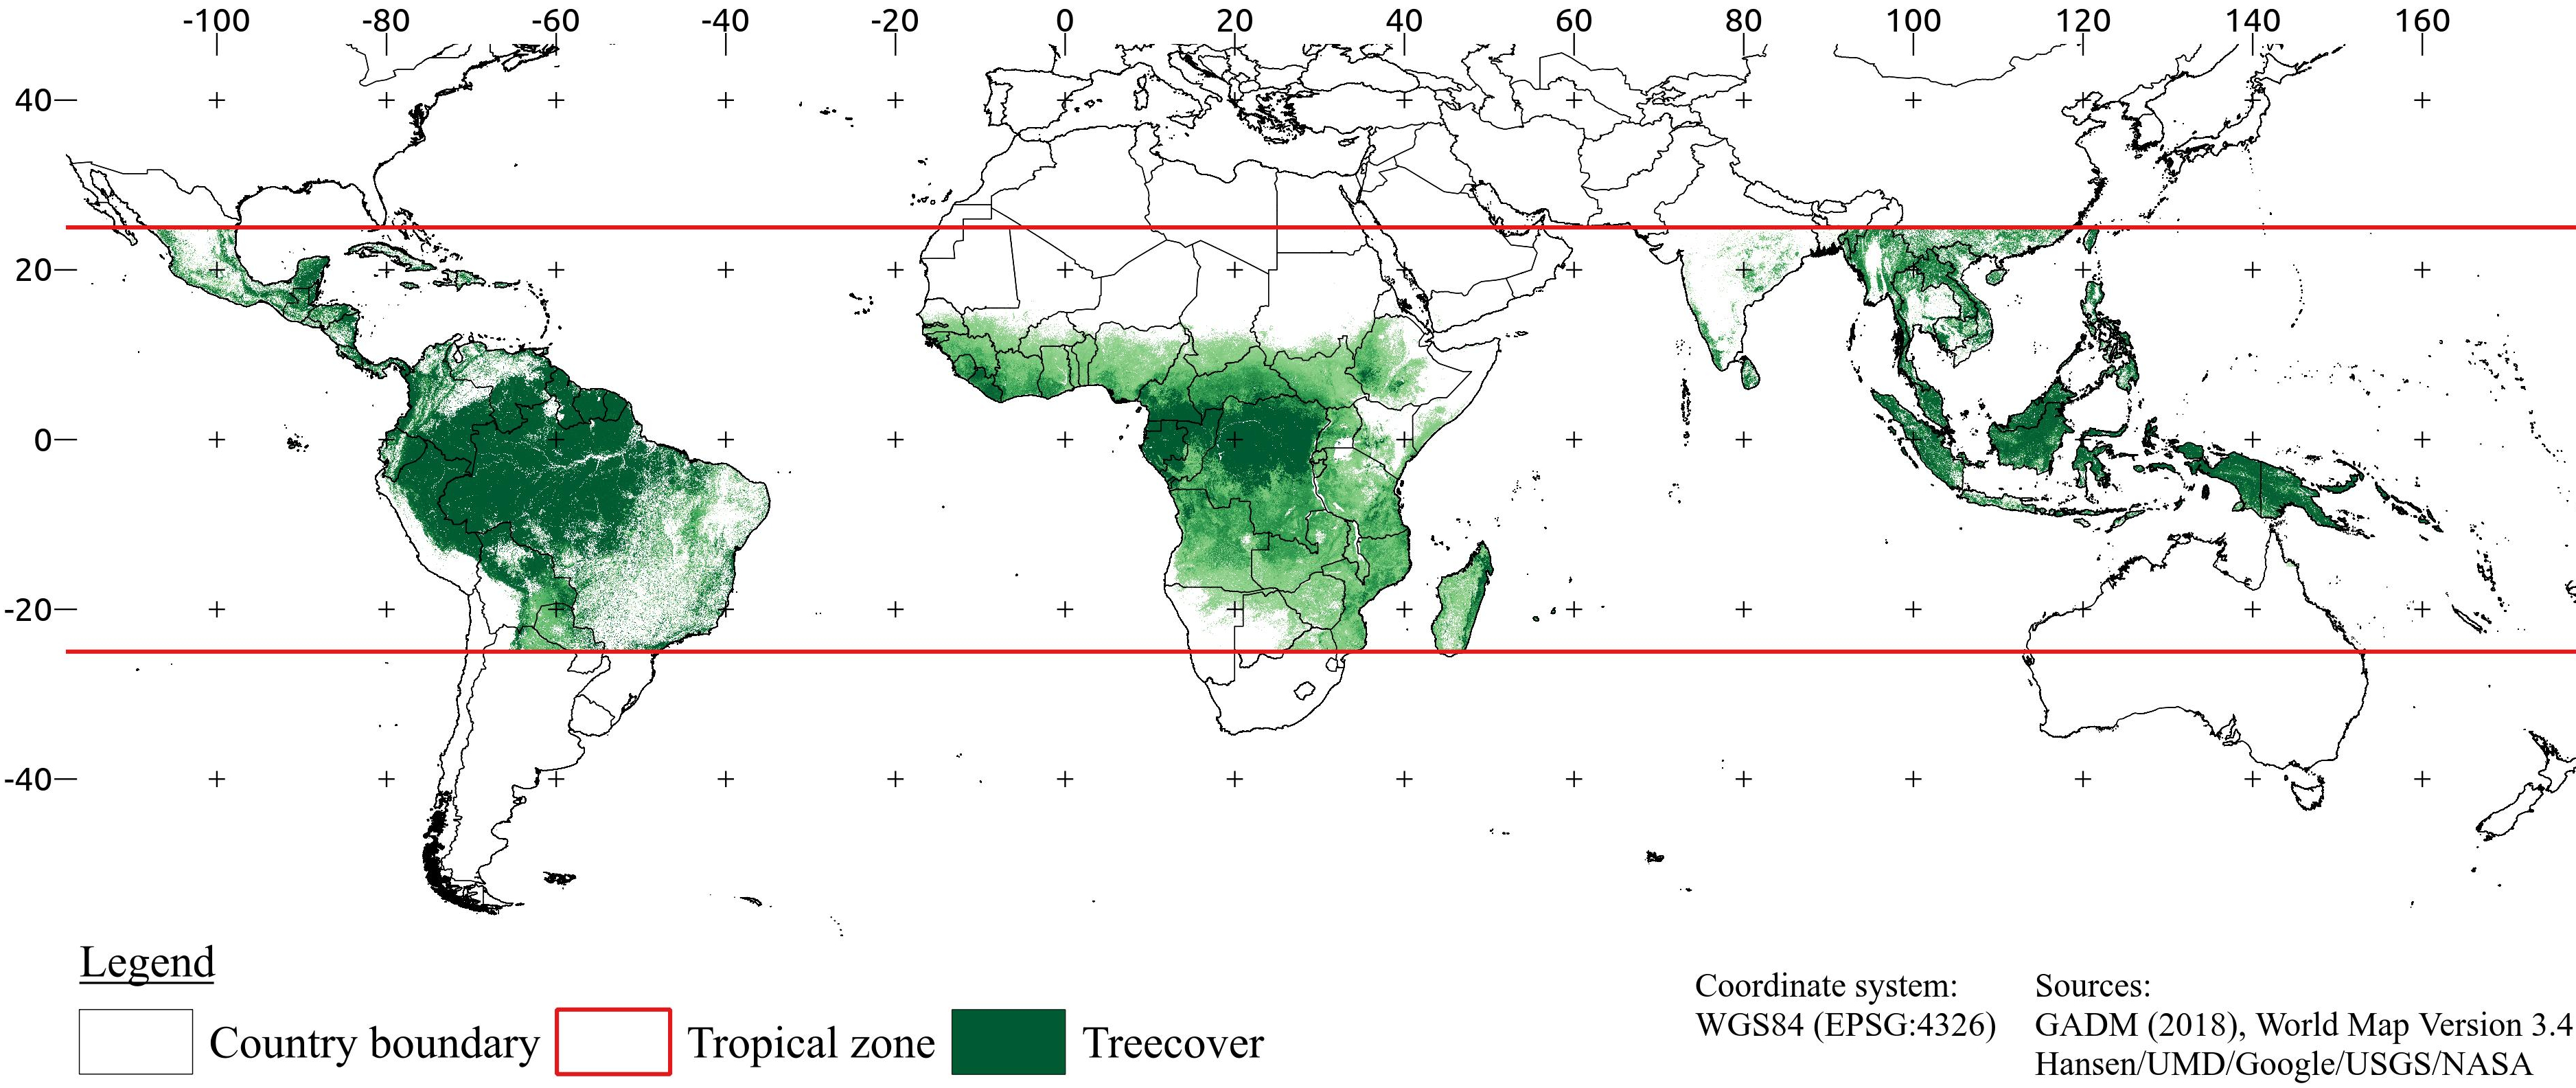
\includegraphics[scale=0.97]{img/intro_overview_frameless}
%		\caption[Tropical zone]{Geographic tropical zone framed red and the tropical forest}
%		\label{fig:tropicalzone}
%	\end{figure}
%	\begin{figure}[ht]
%		\centering
%		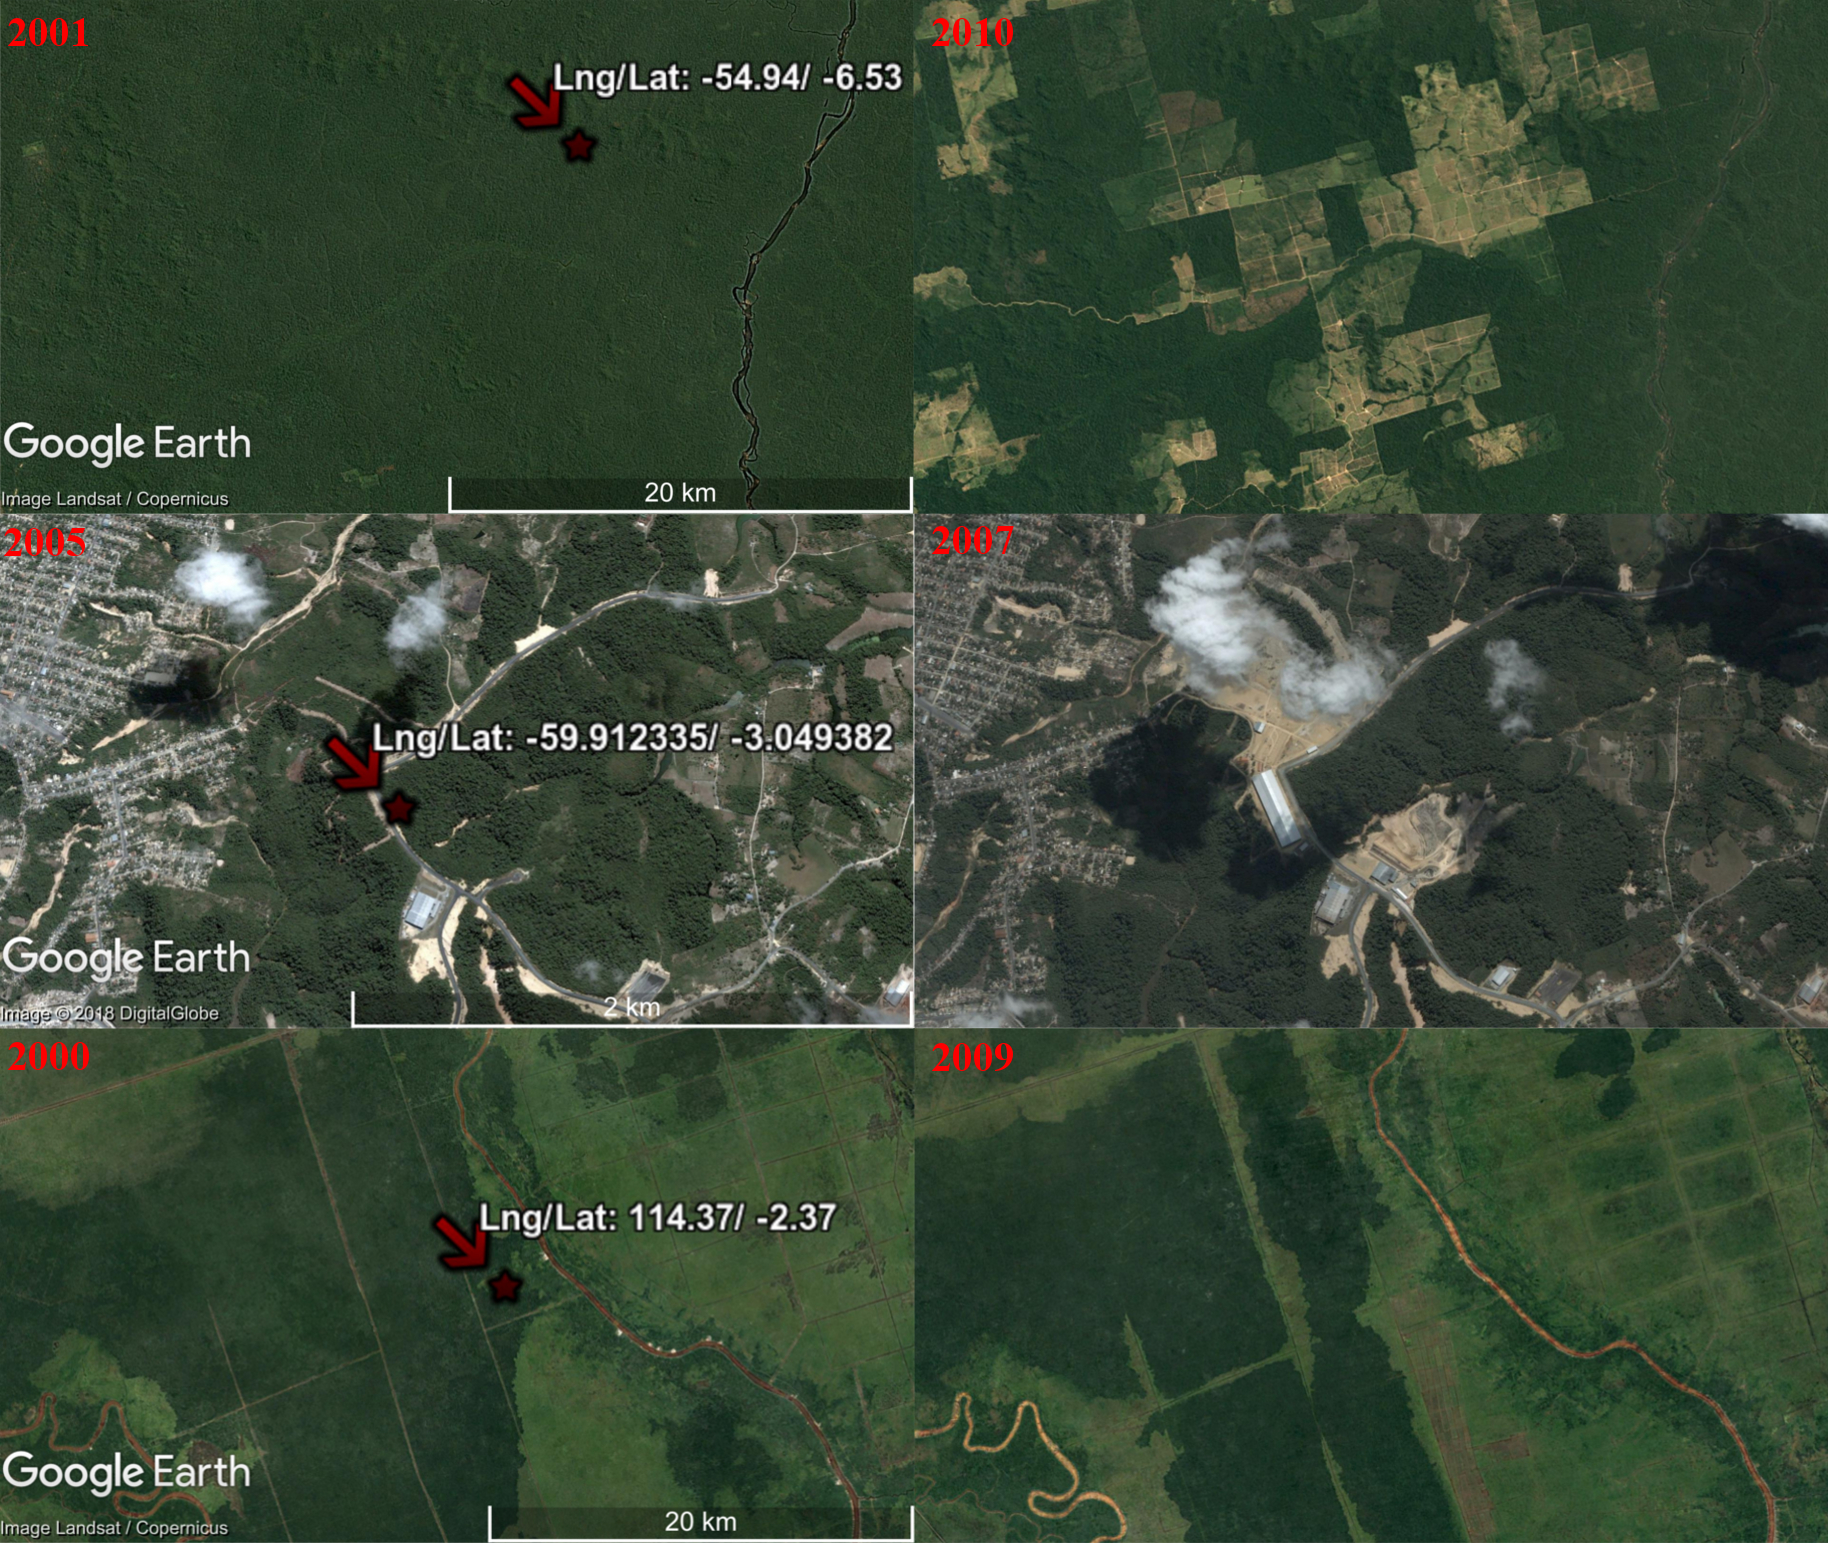
\includegraphics[scale=0.6]{img/deforestation_examples}
%		\caption[Deforestation examples]{Upper Brazil agriculture, middle Brazil urbanization, lower Indonesia large scale palm oil plantations}
%		\label{fig:deforestationexamples}
%	\end{figure}

	\section{Emissions}
	\label{sec:deforestation}


	\section{Ecosystem services}
	\label{sec:ecosystem_services}
	%TODO gaps contribution of deforestation drivers to ghg emissions
	%TODO gaps soil organic carbon emissions

	\begin{itemize}
		\item Different studies on esv change for global and regional scale \citep{Song2018,Costanza2014,Sannigrahi2018}
		\item But no study exclusively focused on the impact of proximate deforestation driver on the esv in tropics
		\item further till now only the loss of monetary value of tropical forest is estimated, no dynamics
		\item because every transition to new land cover produces also a value
		\item we use our proximate deforestation map to estimate these values 
	\end{itemize}
